% \documentclass[a4paper,10pt,draft]{thesis}
\usepackage{physics,amsmath, amsfonts, siunitx, amssymb, graphicx, slashed,subcaption}
\usepackage[utf8]{inputenc}
\usepackage[margin=1in]{geometry}
\usepackage[hidelinks]{hyperref}
\usepackage{xr-hyper}
\newcommand{\n}[1]{\nu_{#1}}
\newcommand{\na}{\nu_\alpha}
\newcommand{\nb}{\nu_\beta}
\newcommand{\ana}{\bar{\nu}_\alpha}
\newcommand{\an}[1]{\bar{\nu}_{\text{#1}}}
\newcommand{\anb}{\bar{\nu}_\beta}
\renewcommand{\a}{\alpha}
\renewcommand{\b}{\beta}
\newcommand{\ab}{\alpha\beta}


\renewcommand{\ne}{\nu_e}
\newcommand{\nm}{\nu_\mu}
\newcommand{\nt}{\nu_\tau}
\newcommand{\ns}{\nu_s}

\newcommand{\ane}{\bar{\nu}_e}
\newcommand{\anm}{\bar{\nu}_\mu}
\newcommand{\ant}{\bar{\nu}_\tau}
\newcommand{\ans}{\bar{\nu}_s}

\newcommand{\nee}{\nu_e \to \nu_e}
\newcommand{\nem}{\nu_e \to \nu_\mu}
\newcommand{\net}{\nu_e \to \nu_\tau}
\newcommand{\nes}{\nu_e \to \nu_s}

\newcommand{\nme}{\nu_\mu \to \nu_e}
\newcommand{\nmm}{\nu_\mu \to \nu_\mu}
\newcommand{\nmt}{\nu_\mu \to \nu_\tau}
\newcommand{\nms}{\nu_\mu \to \nu_s}



\newcommand{\Pee}{P_{e  e}}
\newcommand{\Pem}{P_{e  \mu}}
\newcommand{\Pet}{P_{e  \tau}}
\newcommand{\Pes}{P_{e  s}}

\newcommand{\Pme}{P_{\mu  e}}
\newcommand{\Pmm}{P_{\mu\mu}}
\newcommand{\Pmt}{P_{\mu  \tau}}
\newcommand{\Pms}{P_{\mu  s}}


\newcommand{\Pte}{P_{P_{\tau e}}}
\newcommand{\Ptm}{P_{\tau  \mu}}
\newcommand{\Ptt}{P_{\tau  \tau}}
\newcommand{\Pts}{P_{\mu  s}}

\newcommand{\Paeae}{P_{\bar{e}  \bar{e}}}
\newcommand{\Paeam}{P_{\bar{e}  \bar{\mu}}}
\newcommand{\Paeat}{P_{\bar{e}  \bar{\tau}}}
\newcommand{\Paeas}{P_{\bar{e}  \bar{s}}}

\newcommand{\Pamae}{P_{\bar{\mu}  \bar{e}}}
\newcommand{\Pamam}{P_{\bar{\mu}  \bar{\mu}}}
\newcommand{\Pamat}{P_{\bar{\mu}  \bar{\tau}}}
\newcommand{\Pamas}{P_{\bar{\mu}  \bar{s}}}


\newcommand{\Patae}{P_{\bar{\tau}  \bar{e}}}
\newcommand{\Patam}{P_{\bar{\tau}  \bar{\mu}}}
\newcommand{\Patat}{P_{\bar{\tau}  \bar{\tau}}}
\newcommand{\Patas}{P_{\bar{\mu}  \bar{s}}}

\renewcommand{\th}[1][]{%
  \theta\ifx\\#1\\\else_\text{#1}\fi
}
\newcommand{\thm}[1][]{%
  \theta^\text{M}\ifx\\#1\\\else_\text{#1}\fi
}
\renewcommand{\t}[1]{\text{{#1}}}
\newcommand{\avg}[1]{\left\langle {#1} \right \rangle}
\newcommand*{\dm}[1][]{%
  \Delta m^2\ifx\\#1\\\else_\text{#1}\fi
}
\newcommand{\zreco}{\cos{(\theta_z^{reco})}}
\newcommand{\ztrue}{\cos{(\theta_z^{true})}}
\newcommand{\z}{\cos{(\theta_z)}}
\newcommand{\Ereco}{E^{reco}}
\newcommand{\Etrue}{E^{true}}
\newcommand{\Aeff}{A^\text{eff}}
\newcommand{\emm}{\epsilon_{\mu\mu}}
\newcommand{\emt}{\epsilon_{\mu\tau}}
\newcommand{\eet}{\epsilon_{e\tau}}
\newcommand{\eem}{\epsilon_{e\mu}}
\newcommand{\ett}{\epsilon_{\tau\tau}}
\newcommand{\ep}{\epsilon^\prime}
\begin{document}
\begin{figure}[!h]
    \centering
    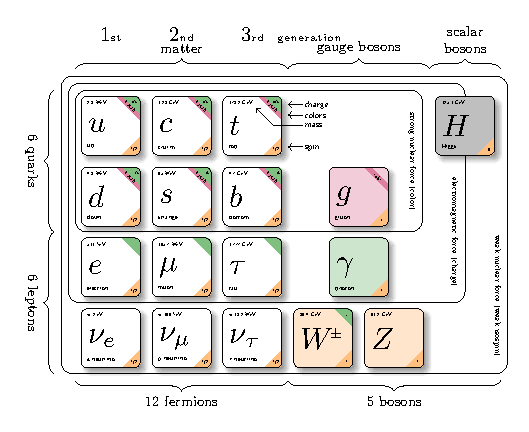
\includegraphics[width=0.7\textwidth]{figures/SM_figure.pdf}
\end{figure}
\section{The Standard Model}\label{ch:SM}
In order to describe the three quantizable forces of nature, we gather the mediators of each force -- the vector bosons -- into local (gauge) symmetry groups. 
Each vector boson has one corresponding generator, the set of which constitutes the group.
The strong charge is mediated by eight massless gluons, which correspond to the eight generators of $\text{SU}(3)_C$. 
The weak charge is mediated by the three massive gauge bosons $W^\pm$ and $Z$, and the massless photon $\gamma$, 
which constitute the generators of $\text{SU}(2)_L$ and $\text{U}(1)_Y$. 

The subscript of each group denotes by which mechanism that force is mediated. The gluons mediate the strong force through interactions of color, emphasized with subscript $C$. The weak force only sees left-handed particles, 
which we distinguish with the subscript $L$. And the electroweak interaction that a particle undergoes is determined by its hypercharge $Y$. For example, the quarks all have a nonzero color and hypercharge, 
so they participate in the strong and electromagnetic interactions. If a quark is left-handed, it will also feel the weak interaction. The neutrinos on the other hand, have neither charge nor color, 
so they are insivible to both the strong and electromagnetic force. We express this by letting their fields transform as singlets under those symmetry groups.

Together, these three interactions make up the Standard Model gauge group $\mathrm{SU}(3)_{\mathrm{C}} \times \mathrm{SU}(2)_{L} \times \mathrm{U}(1)_{Y}$. 
This determines the form of the three coupling constants, but which numerical values must be experimentally measured. 
Since the vector bosons are represented by the generators, they are uniquely determined by the symmetry group. However, the scalar boson(s) and fermions are free as long as they
belong to representations of the symmetry group. By this construction, the fermions have more degrees of freedom with which we can propose amendments to the model with. Even the
number of fermions must be experimentally verified and can be altered from a phenomenological standpoint. In this work,
we will use this leniency to make drastic modifications to the Standard Model fermions and examine to which extent 
these modifications might be supported by experimental evidence.


% \subsection{Lepton mixing}
% Now we shall see how the charged leptons interact with the chargeless neutrinos.
% Consider how charged leptons interact with the Higgs field. In the unitary gauge, the Higgs-lepton Yukawa Lagrangian 
% \begin{align}
%     \label{eq:YukawaLagrangian}
%     \mathcal{L}_{H}=-\left( \frac{v + H}{\sqrt{2}} \right) \ell_{\alpha L}^{\prime} Y_{\alpha \beta}^{\prime \ell} \ell_{\beta R}^{\prime}
% \end{align}
% has a non-diagonal Yukawa coupling matrix $Y^{\prime \ell}$, which results in the charged lepton masses being non-definite. This can be remedied by diagonalizing $Y^{\prime \ell}$ with a unitary matrix $V^\ell$
% \begin{align}\label{eq:leptonYukawaDiag}
%     V_{L}^{\ell \dagger} Y^{\prime \ell} V_{R}^{\ell}=Y^{\ell}\,.
% \end{align}
% This procedure give the charged lepton fields $\ell_{X}=V_{X}^{\ell \dagger} \ell_{X}^{\prime}$ definite mass. 
% However, this alters the form of the neutral and charged current interactions, which the neutrinos undergo. The leptonic charged weak current now takes the form
% \begin{align}
%     \label{eq:j_CC}
%     j^\rho_W &= 2 \bar{\nu}^\prime_\alpha \gamma^\rho \ell^\prime_\alpha \nonumber \\
%              &= 2 \bar{\nu}_\alpha V^{\ell \dagger} \gamma^\rho V^\ell \ell_\alpha \nonumber \\
%              &= 2 \bar{\nu}_\alpha \gamma^\rho \ell_\alpha\,,
% \end{align}
% where each lepton field and matrix have an implied $L$ subscript, which was dropped for clarity. The flavor neutrino fields $\nu_\alpha$ now only couple to the associated charged lepton field $\ell_\alpha$. However, 
% $\nu_\alpha$ remained massless, since no flavor rotation $V^{\ell \dagger}$ can make massless fields massive.
% \bibliographystyle{apalike}
% \bibliography{ref}
% \end{document}